% Latex Beamer template following CERN template guidelines (or trying!)

\documentclass[aspectratio=169]{beamer}
\usepackage{xcolor}
\usepackage{graphicx}
\usepackage{multicol}
\usepackage{tikz}

\usetheme{CERN}

% Talk date
% Uncomment this to define a presentation date distinct from \today
% \def\mydate{20 Feb 2000}

% Preamble
\title[]{Title}
\subtitle{Subtitle}
\author[Author]{\texorpdfstring{\url{name.surname@cern.ch}}{Author}}

% Body
\begin{document}
    
    \cernSplashBlue

    % Title
    {
    \setbeamertemplate{footline}{}
    \setbeamertemplate{navigation symbols}{}
    \frame{\titlepage}
    }
    \setcounter{framenumber}{0}

    % TOC
    \frame{
        \frametitle{Table of Contents}
        \begin{multicols}{2}
            \tableofcontents
        \end{multicols}
    }



    \section{Introduction}
    \frame{
        \frametitle{Table of Contents}
        \begin{multicols}{2}
        \tableofcontents[
            currentsection,
            sectionstyle=show/shaded,
            ]
        \end{multicols}
    }

    \frame{
        \frametitle{This is the first slide}
        %Content goes here
        \begin{block}{Ideas}
            See how this loooks
        \end{block}
        \begin{itemize}
            \item Item 1
            \item Item 2
        \end{itemize}
    }

	% This block includes a picture full slide
	{ % all template changes are local to this group.
		\setbeamertemplate{navigation symbols}{}
		\begin{frame}[plain]
			\begin{tikzpicture}[remember picture,overlay]
			\node[at=(current page.center)] {
				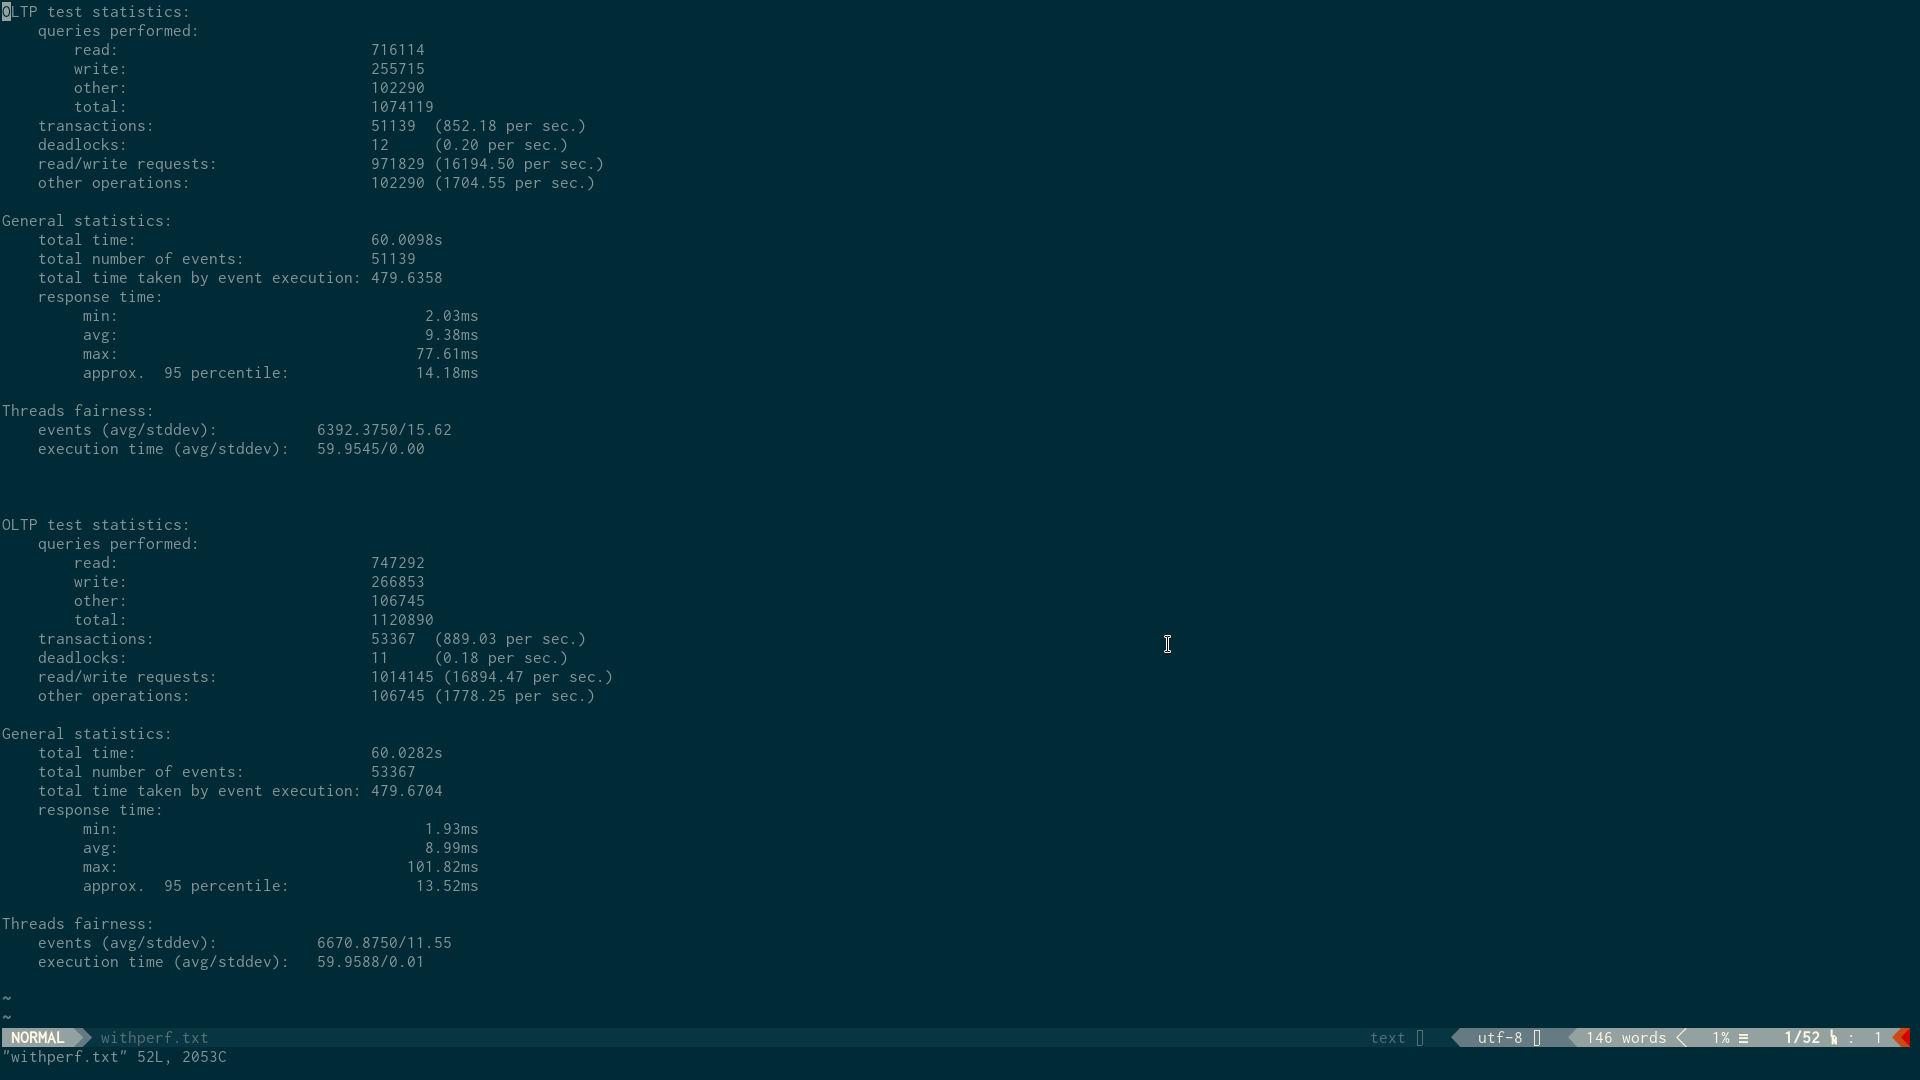
\includegraphics[width=\paperwidth]{images/image.png}
			};
			\end{tikzpicture}
		\end{frame}
	}

    \subsection{Intro subsection}
    \frame{
        \frametitle{This is the second slide}
        \framesubtitle{A bit more information about this}
        %More content goes here
        \begin{alertblock}{Alert block}
            Alert text
        \end{alertblock}
    }
    
    \section{Section 1}
    \frame{
        \frametitle{Table of Contents}
        \begin{multicols}{2}
        \tableofcontents[
            currentsection,
            sectionstyle=show/shaded,
            ]
        \end{multicols}
    }

    \frame{
        \frametitle{Generic slide}
        \framesubtitle{A bit more information about this}
        %More content goes here
    }
    \section{Section 2}
    \frame{
        \frametitle{Table of Contents}
        \begin{multicols}{2}
        \tableofcontents[
            currentsection,
            sectionstyle=show/shaded,
            ]
        \end{multicols}
    }
    \frame{
        \frametitle{Generic slide}
        \framesubtitle{A bit more information about this}
        %More content goes here
    }

    
    \section{Conclusion}
    \frame{
        \frametitle{Table of Contents}
        \begin{multicols}{2}
        \tableofcontents[
            currentsection,
            sectionstyle=show/shaded,
            ]
        \end{multicols}
    }
    
    \frame{
        \frametitle{Generic slide}
        \framesubtitle{A bit more information about this}
        %More content goes here
    }
    
    \section{Acknowledgements}
    \frame{
        \frametitle{Table of Contents}
        \begin{multicols}{2}
        \tableofcontents[
            currentsection,
            sectionstyle=show/shaded,
            ]
        \end{multicols}
    }
    \frame{
        \frametitle{Generic slide}
        \framesubtitle{A bit more information about this}
        %More content goes here
    }

    \section{}
    \cernSplashWhite

\end{document}

